
\section{Methods}
\label{sec:methods}


%There are several approaches we consider. 

%We propose several methods that we group into 2 major classes: segment methods and hierarchical methods. 
%We subdivide the segment methods into word-level methods and phrase-level methods. 
%There are two features of semantic vector space embeddings that we use to design our methods. 
%The vector space embeddings come with an associated similarity measure. 
%The methods that use this feature we will call similarity methods. 
%The vector space embeddings can also be used to generate a list of vectors in a neighborhood of a given vector. 
%The vectors in the neighborhood can be ranked by their similarity to the given vector. 
%We use this feature to generate extra references for a  given reference.
%Methods that use this feature we will call generation methods. 

Before we describe the methods we used in this work, we give a classification of the approaches that could be used to attack the pocity of references problem. 
We group the approaches into 2 major classes: segment methods and hierarchical methods.
The hierarchical methods use a parse tree to compose word vectors into phrase vectors and phrase vectors into sentence vectors. 
We will not deal with hierarchical approaches in this paper. 
We subdivide the segment approaches into word-level methods and phrase-level methods. 
Each of these approaches can be further  classified into two more classes depending on how we use the vector space embedding. 
There are two features of semantic vector space embeddings that we use to design our methods. 
The vector space embeddings come with an associated similarity measure. 
One class of approaches assigns a similarity to references. 
The methods that use this feature we will call similarity methods. 
The similarity measure associated with vector space embeddings can also be used to generate a list of vectors in a neighborhood of a given vector. 
The vectors in the neighborhood can be ranked by their similarity to the given vector. 
We use this feature to generate extra references for a  given reference.
Methods that use this feature we will call generation methods. 
In this paper we only report on segment similarity methods 

We single out three similarity methods and we name them SLEU, VLEU, and XLEU for scalar, vector, and cross BLEU. 
SLEU is a word similarity metric. 
VLEU and XLEU are phrase similarity metrics. 

%Word Level
%
%The bleu algorithm loops over the ngrams in the system output and the reference transcriptions. 
%A match count is accumulated for the precision computation. 
%A one is added to the count if the system and reference ngrams match and a zero is added otherwise. 
%The simplest of our approaches computes the similarity between the system output and reference words and adds this number instead of a one or a zero to the match count used in the precision calculation. 

\begin{figure}
  \centering
  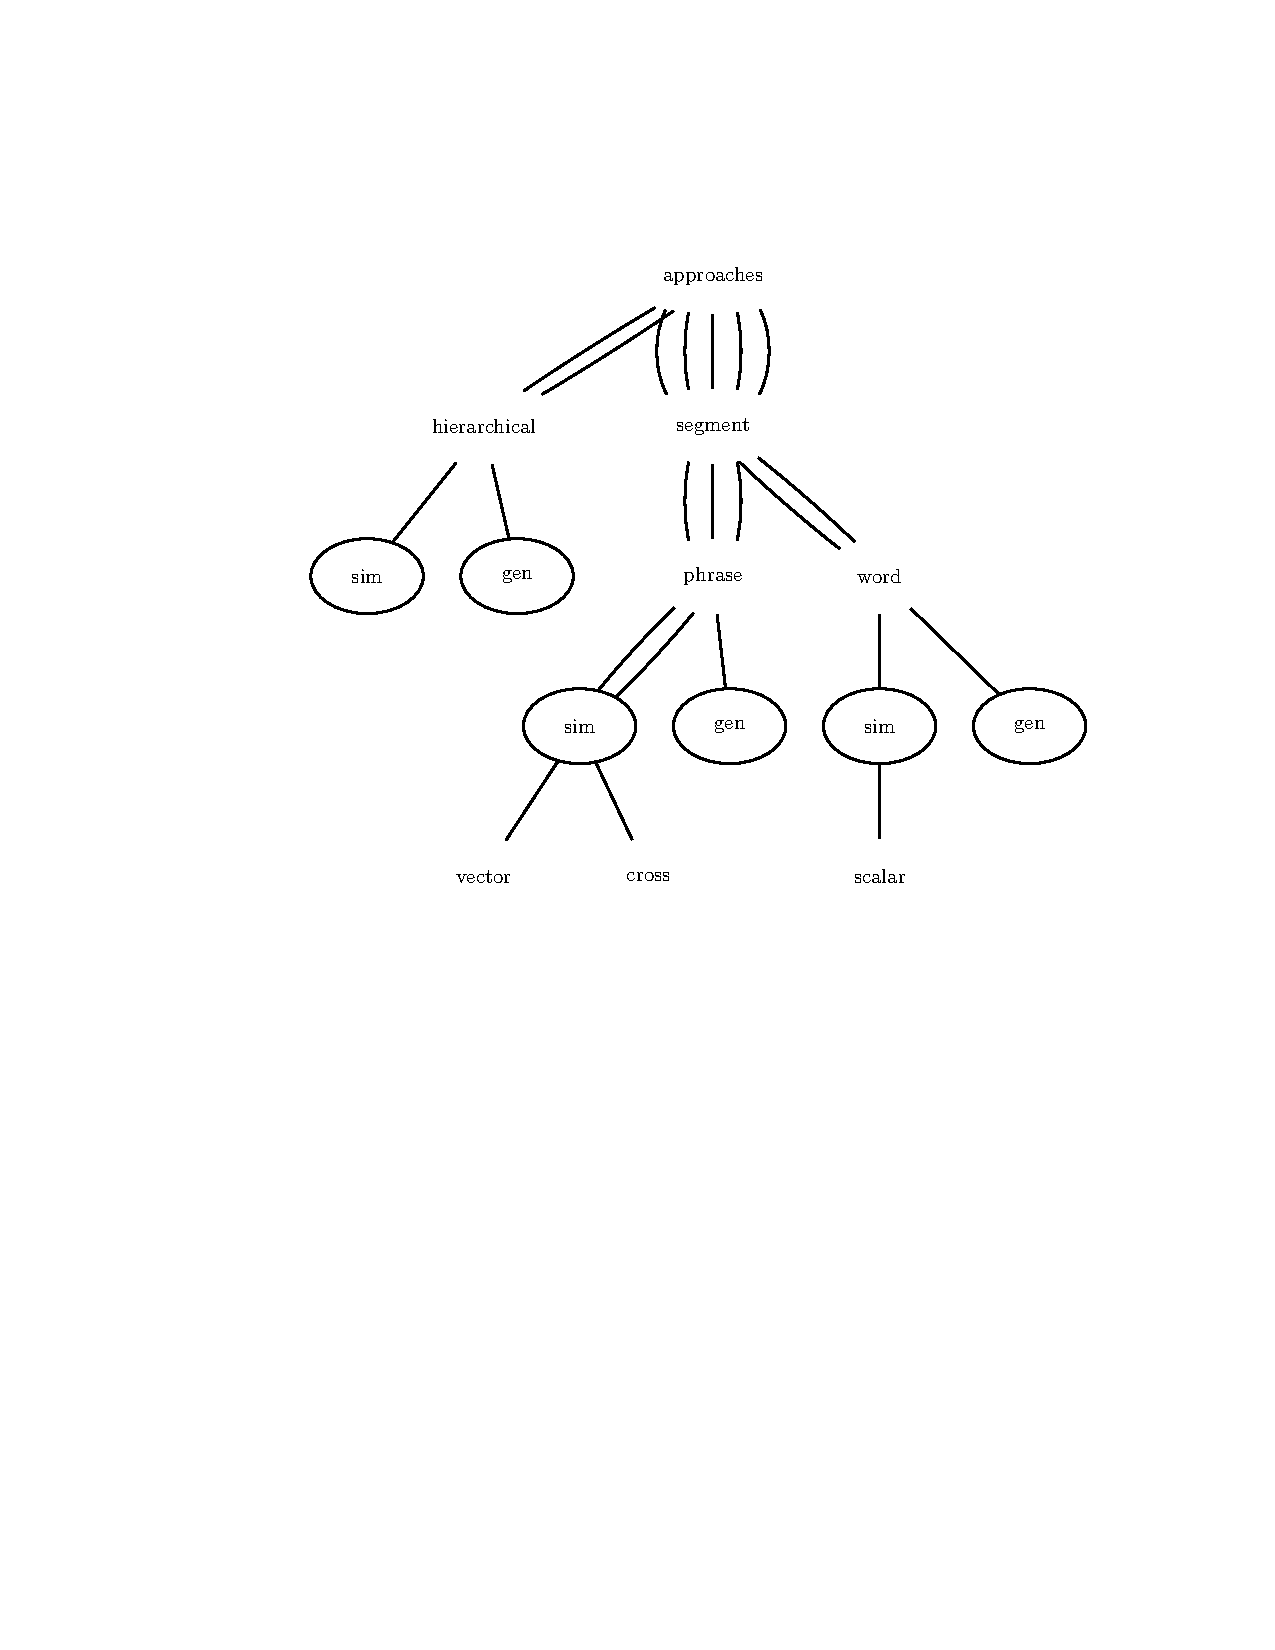
\includegraphics[width=\linewidth,height=2.0181in]{approaches.pdf}
  \caption{Possible approaches for incorporating semantic vectors into an evaluation metric.}
  \label{fig:approaches}
\end{figure}


The BLEU algorithm loops over the ngrams in the system output and the reference transcriptions. 
A match count is accumulated for each of the four precision computations. 
A one is added to the count if the system and reference ngrams match and a zero is added otherwise. 
All three methods, SLEU, VLEU, and XLEU compute the similarity between the system output and reference $n$grams and adds this number instead of a $1$ or a $0$ to the match count used in the precision calculation. 
SLEU only adds similarity scores for $1$grams. 
VLEU adds similarity scores for $1$ to $1$, $2$ to $2$, $3$ to $3$,  and $4$ to $4$ grams. 
XLEU adds similarity scores for $1$ to $1$, $2$ , $3$, and $4$-grams, $2$ to $1$, $2$, $3$, and $4$-grams, $3$ to $1$, $2$, $3$, $4$- grams, and $4$ to $1$, $2$, $3$, $4$-grams. 

%Another  approach works by starting with words or phrases from MT system output and a list of synonyms or meaning equivalent phrases are produced together with the distances between them. 
%If one of these synonyms matches the reference word being considered then its associated distance is added in the precision computation . 
%A third approach works similarly but instead  starts with words and phrases extracted from a reference translation and a list of its closest synonyms or meaning equivalent phrases are produced. 
%If one of these synonyms matches the system output word being considered then it is added in the precision computation weighted by its associated distance. 
%Next we discuss the method we use to obtain synonyms and how we can measure synonomy. 

%The traditional BLEU metric measures the overlap of n-grams from the decoder output with n-grams from the reference corpus sentences. 
%Credit is given to the decoder output n-gram only when there is an exact string to string match. 
%If the reference sentence was:
%The boy went to the store
%But the decoder output:
%The boy went to the supermarket
%BLEU would assign no credit to the 1-gram supermarket. 
%Although supermarket does not deserve the full creditof 1 given to store by BLEU, it seems harsh to give it no credit at all. 
%Word2vec might place supermarket in a neighborhood of store where the two words have vectors that have a cosine angle of 0.2 between each other. 
%Our algorithm would assign 0.2 instead of 0 to the word supermarket.
%We do this until we find a match for a small number (k = 3) of words in a neighborhood of the 1-gram in the reference 1-gram. For n-grams with n > 1 the
%algorithm is slightly more complicated. 
%We first discard decoder output n-grams that differ by more than a single word. 
%Then we consider the n-grams that result by replacing the word that differs with words close to it as above. 
%Again we do this up to k = 3 times for the top k words that appear in the neighborhood of the differing word in the reference transcription.

Our simplest method, SLEU,  only differs from BLEU in the precision computation for $1$grams. 
When a candidate $1$gram does not match any $1$gram in the reference, we compute the similarities with each of the remaining $1$grams in the reference. 
Instead of adding $0$ to our match count, we add the maximum of these similarities. 
We then remove one instance of the $1$gram that yielded the maximum similarity. 
This step of removing the argmax $1$gram is done to mitigate the overgeneration problem. 
In the discussion section we consider a problem that this step causes and for which we do not yet have a solution. 

We consider the $1$gram case separately, because it has a stronger theoretical basis. 
The similarities are given to us by word2vec. 
We used the pre-trained vectors available for download on the word2vec webpage. 
These aare $300$ dimensional vectors. 
The vector space embedding performed by word2vecd operates on $1$grams. 
Similarities for higher $n$grams are computed and we exploit this in our phrase-level methods, VLEU and XLEU, but we see this as having weaker theoretical foundations. 

VLEU is similar to SLEU; when a system output $n$gram does not match exactly with any reference $n$gram, its similarity with the remaining $n$grams is computed and the maximum of these similarities is added to the match count. 
XLEU computes yet more similarities. 
The similarity measure that operates on the embedded word vectors allows the similarity between $j$grams and $k$grams for $j$ different from $k$ to be computed. 
For a non-exact matching $j$gram we compute similarities with $k$grams for $k$ between $1$ and $4$. 
We add the maximum of these similarities to our match count. 

Note that when computing precision, we need to divide by the total number of possible matches. 
What is that number in the XLEU case?
If we compute similarities with all possible reference $n$grams and not just the ones remaining, we should divide by the total number of $n$grams. 
All the $n$grams have a chance of matching or being similar to all the $n$grams. 
But if we only consider similarities with the remaining $n$grams it is not as clear what the denominator in the precision computation should be. 
This makes a large difference in the final score. 

%We do this until we find a match for a small number (k = 3) of words in a neighborhood of the 1-gram in the reference 1-gram. 
%For n-grams with n > 1 the algorithm is slightly more complicated. 
%We first discard decoder output n-grams that differ by more than a single word. 
%Then we consider the n-grams that result by replacing the word that differs with words close to it as above. 
%Again we do this up to k = 3 times for the top k words that appear in the neighborhood of the differing word in the reference transcription.

% Phrase Level
% Sentence Level
%We will use the Socher and Iyyer composition methods to generate candidate ngrams of higher order that aare similar in meaning to the system output. 


\subsection{Data}
\label{sec:data}

%We test the metrics on the WMT13 corpus. 
%This corpus consists of $3000$ segment pairs. 
%Each pair consists of a system output and one reference. 
%The system output has 55786 tokens
%The reference has 56089 tokens. 

We test the metrics on three standard corpora and an artificial corpus.

\subsubsection{Standard Corpora}
\label{sec:standardcorp}

The WMT13 German to English corpus consists of $3000$ segment pairs. 
Each pair consists of a system output and one reference. 
The system output has 55786 tokens, the reference has 56089 tokens. 

\subsubsection{Artificial Corpus}
\label{sec:artificial}

We generated a small corpus of sentence pairs with simple structure. 
We wantted to create a corpus of segment pairs that were very close in meaning. 

\begin{table}[h]
  \centering
  \begin{tabular}{|c|c|c|}
    candidate & ||| & reference \\
\hline
the person went by the supermarket & ||| & a person ran to a store \\
the girl ran by the store & ||| & we drove by the store \\
the woman drove to a supermarket & ||| & a girl went around the store \\
the girl drove to a mall & ||| & we went around the supermarket \\
the girl ran to a mall & ||| & she ran to a supermarket \\
a boy went by a supermarket & ||| & they walked by the mall \\
the boy drove to the store & ||| & we ran by the supermarket \\
the woman drove by a supermarket & ||| & a girl walked to a mall \\
the woman ran around the mall & ||| & they went by the mall \\
the person walked to a store & ||| & she walked around a mall \\
\hline
  \end{tabular}
  \caption{Some examples of sentences from an artificial corpus.}
  \label{tab:sentencexamples}
\end{table}

\begin{table}
  \centering
  \begin{tabular}{|c|c|c|c|c|}
\hline
sleu & 1227.68 & 238.0 & 62.0 & 10.0 \\
vleu& 1227.68 397.09 & 182.42 & 85.73 \\
xleu	& 1052.11 & 632.47 & 437.74 & 283.26 \\
\hline
  \end{tabular}
  \caption{Total number of $n$-grams in artificial corpus.}
  \label{tab:artificialtotalngrams}
\end{table}
\begin{table}[h]
  \centering
  \begin{tabular}{|l||c|c|c|c|}
    \hline
metric & $1$-grams & $2$-grams & $3$-grams & $4$-grams \\
BLEU SLEU VLEU & 56089 &  53089 & 50105 & 47138 \\
XLEU & 159283 & 159267 & 159216 & 159060 \\
\hline
  \end{tabular}
  \caption{Total $n$grams in the WMT13 corpus.}
  \label{tab:totalngrams}
\end{table}


%%% Local Variables: 
%%% mode: latex
%%% TeX-master: "ling848fall2014"
%%% End: 
